\section{Machine Learning Workflow} \label{sec:MLWF}
Als \gls{Machine Learning Workflow} wird der systematische Prozess zur Entwicklung, Evaluierung und Anwendung von Algorithmen des \glsdisp{ML}{maschinellen Lernens} bezeichnet. In der Literatur werden auch Bezeichnungen wie \textit{Machine Learning Pipeline} oder \textit{Data Science Pipline} verwendet. Die Strukturierung eines Workflows sorgt für Übersichtlichkeit, Effizienz, Reproduzierbarkeit und Skalierbarkeit von Anwendungen des \glsdisp{ML}{maschinellen Lernens}. Die Komponenten des \gls{Machine Learning Workflow}[s] sind nicht immer einheitlich. Nicht alle Prozessschritte sind für jedes Projekt notwendig. In \cite{Biswas.2022} wird versucht, die üblichen Prozessschritte zu definieren. In diesem Kapitel werden die Komponenten vorgestellt, welche Relevanz für diese Arbeit besitzen. Die Abbildung \ref{fig:MLWorkflow} stellt den \gls{Machine Learning Workflow} grafisch dar.

\begin{figure}[htb]
    \centering
    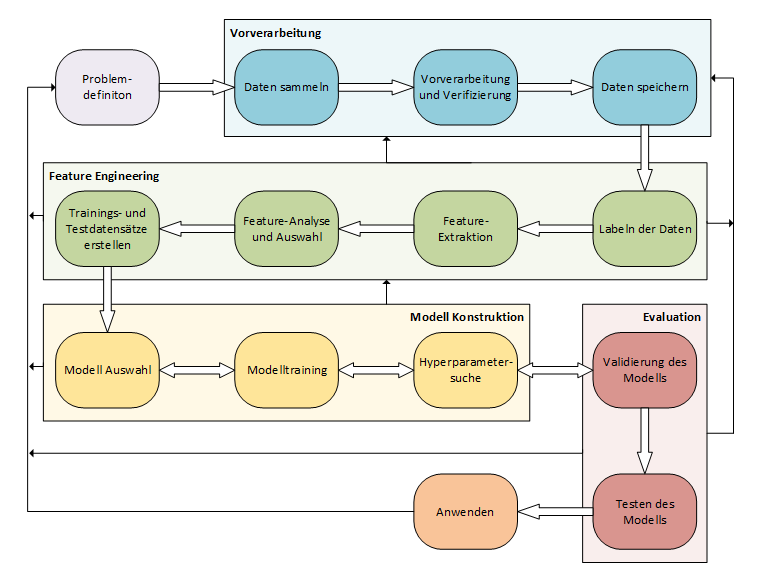
\includegraphics[width=\textwidth]{img/Grafiken/Machine Learning Workflow.png}
    \caption[Der Machine Learning Workflow]{Der \gls{Machine Learning Workflow} und seine Prozessschritte.}
    \label{fig:MLWorkflow}
\end{figure}


In der Grafik \ref{fig:MLWorkflow} sind Rückführungen zu früheren Prozessschritten zu sehen. Dadurch entstehen Schleifen. Einige dieser Schleifen sind optional und nur notwendig, wenn bspw. Testergebnisse sehr unbefriedigend sind. Ein Beispiel hierfür ist die Rückkehr zur Problemdefinition. Andere Schleifen sind übliche Praxis bei der Erstellung von Anwendung mit \glsdisp{ML}{maschinellem Lernen}. Z.B. ist die Suche von \gls{Hyperparameter} immer mit der Rückkehr zum Training verbunden \cite{Biswas.2022, Zheng.2018, Zheng.2015, Elshawi.2019}. 

\subsection{Problemdefinition und Vorverarbeitung}

\textbf{Problemdefinition}\par
Ziel des \gls{Machine Learning Workflow}[s] ist es, eine Anwendung zu erstellen, welche ein spezifisches Problem löst. Das die klare Definition einer Aufgabe, ein elementarer Schritt ist von Algorithmen des \glsdisp{ML}{maschinellen Lernens}, ist in \autoref{sec:Grundlagen ML} verdeutlicht. Die klare Definition ist auch hilfreich für den Erwerb von Fachwissen im Bereich der Aufgabe. Dies kann für den weiteren verlauf des Workflows nützlich sein \cite{Biswas.2022, Zheng.2018, Nielsen.2020}. \dubpar

\textbf{Sammeln von Daten} \label{sec:Worflow DatSam}\par
Ein Modell benötigt Daten für das Training. In diesem Schritt geht es darum, Rohdaten zu sammeln, die relevant sind für die Aufgabe, um diese weiterzuverarbeiten. Je nach Aufgabe ist dieser Prozess unterschiedlich aufwendig \cite{Biswas.2022, Elshawi.2019}. \dubpar

\textbf{Vorverarbeitung der Daten}\par
Die gesammelten Rohdaten können uneinheitlich sein. Sollen bspw. Daten aus mehreren Abteilungen einer Firma verwendet werden, um ein Modell zu erstellen, kann es sein, dass Abteilung \(A\) ein anderes Datumsformat benutze als Abteilung \(B\). Auch können Lücken in Daten vorhanden sein. Solche Probleme sind zu filtern und zu bereinigen \cite{Biswas.2022, Elshawi.2019}. Ebenfalls kann es sinnvoll sein, hier eine Verifikation der Daten vorzunehmen, um sicherzustellen, dass die Rohdaten auch die erwartete Information beinhalten \cite{Shearer.2000}. \dubpar

\textbf{Speicherung der Daten}\par
Frühzeitige Überlegungen zur Speicherung der Rohdaten sind vorteilhaft für den weiteren Verlauf des \gls{Machine Learning Workflow}[s]. Je nach Projekt sind andere Datenformate besser geeignet als andere. Auch der Speicherort ist relevant. Solche Überlegungen sorgen für einen effizienteren Ablauf des \gls{Machine Learning Workflow}[s] \cite{Biswas.2022}. 

\subsection{Labeln der Daten}
Wenn eine \glsdisp{überwachtes Lernen}{überwachte Lernmethode} verwendet werden soll, dann wird ein \gls{Zielvektor} benötigt. Dieser ist i.d.R. manuell zu erstellen. Das kann je nach Datenmenge und Datenart unterschiedlich aufwendig sein \cite{Biswas.2022}. Ein Beispiel aus der Bildverarbeitung ist eine Anwendung, welche Ampeln erkennen soll. In diesem Prozessschritt müssen alle Bilder, die für das Training verwendet werden sollen, mit einem \gls{Label} \textit{Ampel} oder \textit{keine Ampel} versehen werden. 

\subsection{Extraktion und Konstruktion der Features} \label{sec:ML FeatExtr}
Aus den Rohdaten müssen \gls{Feature}[s] kreiert werden, mit denen das Modell lernen kann. Dazu sind Überlegungen anzustellen, welche \gls{Feature}[s] sich aus den Rohdaten extrahieren lassen. Hierbei ist Fachwissen über die Aufgabe und die Rohdaten von großem Vorteil. Dadurch ist es möglich die Nützlichkeit möglicher \gls{Feature}[s] zu beurteilen und auch selbst kreative \gls{Feature}[s] zu entwerfen. Fachwissen wird auch benötigt, um gezielten \gls{Bias} in das Modell einzuführen. Auch ungewollter \gls{Bias} ist mit Fachwissen in manchen Fällen identifizierbar (\autoref{sec:Herausforderungen ML}). Generell ist in diesem Prozessschritt viel Achtsamkeit in Bezug auf \gls{Bias} sinnvoll \cite{Zheng.2018, Geron.2019}. \par

Auch auf \gls{Leakage} ist zu achten. Ein Beispiel wie \gls{Leakage} entstehen kann, ist die Komprimierung von Zeitreihen zu \gls{Feature}[s] (\autoref{sec:sequenzen ML}). Aus der Zeitreihe \(A\) sind komprimierte  \gls{Feature}[s] zu extrahieren, genauso wie aus der Zeitreihe \(B\). Was nicht bemerkt wird ist, dass diese eine zeitliche Überlappung haben. Dadurch sind die komprimierten Datenpunkte zu \(A\) und \(B\) nicht unabhängig voneinander. Das kann dazu führen, dass die Proben im Datensatz zu wenig Varianz aufweisen und das Modell lernt nicht zu \glsdisp{Generalisierung}{generalisieren}. Auch für die Evaluation kann das zu Problemen führen \cite{Zheng.2018, Geron.2019}. \par

Extrahierte \gls{Feature}[s] lassen sich Transformieren. Solche Transformationen zielen meistens auf eine Veränderung der Verteilung ab. Dies kann Modellen helfen aus \gls{Feature}[s] besser zu lernen. \dubpar

\textbf{Gruppierung}\\
Die Werte in einem \gls{Feature} werden in Gruppen eingeteilt. Dies kann durch vom Ersteller gewählte Wertebereiche erfolgen, oder nach statistischen Prinzipien, wie nach Quantilen. Dabei werden die Werte in gleich große Gruppen aufgeteilt. Z.B. werden die Werte bei einer Einteilung nach Perzentile in 100 Gruppen eingeteilt und in jeder befindet sich die gleiche Anzahl an Werten. Die Gruppen sind durchnummeriert. Die Nummer der Gruppe ist das neue konstruierte \gls{Feature} \cite{Zheng.2018}. \dubpar

\textbf{Power Transformationen}\\
Power Transformationen zielen darauf ab, die Varianz innerhalb eines \gls{Feature}[s] zu stabilisieren. Ein Beispiel ist die logarithmische Transformation. \gls{Feature}[werte] die sich über mehrere Größenordnungen verteilen, besitzen eine sehr hohe Varianz. Die Anwendung eines Logarithmus auf diese Verteilung komprimiert den Wertebereich. Dies reduziert die Varianz und erhöht die Vergleichbarkeit der Daten. Die Abbildung \ref{fig:bspLogTrans} veranschaulicht die logarithmische Transformation \cite{Zheng.2018}. 

\begin{figure}[htb]
    \centering
    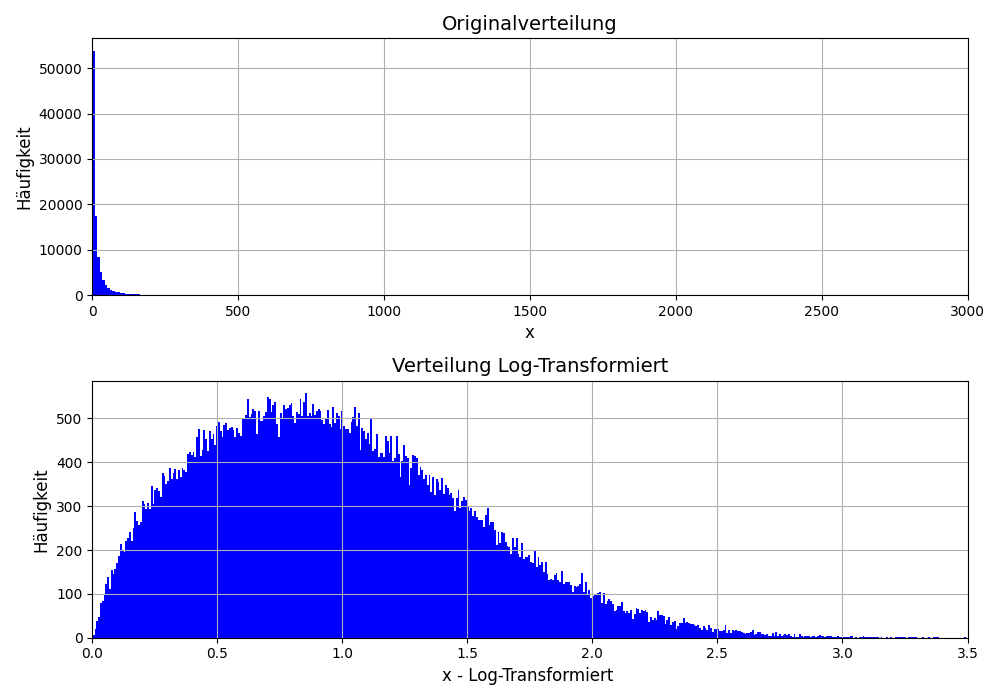
\includegraphics[width=0.9\textwidth]{img/Plots/Log-Transfomation.png}
    \caption[Beispielanwendung der logarithmischen Transformation.]{Beispielanwendung der logarithmischen Transformation. Werte eines \gls{Feature}[s], welche sich über mehrere Größenordnungen verteilen. Die Anwendung des Logarithmus verkleinert den Wertebereich erheblich.}
    \label{fig:bspLogTrans}
\end{figure}

Eine weitere Power Transformation ist die Box-Cox-Transformation. Diese versucht eine Verteilung näher an eine Normalverteilung zu bringen. Dies kann hilfreich sein, da einige Modelle besser mit Normalverteilung umgehen können. Die Formel \ref{eq:BoxCox} zeigt die Rechenvorschrift der Box-Cox-Transformation.

\begin{equation}
    \label{eq:BoxCox}
    x(\lambda) = 
    \begin{cases} 
    \frac{x^\lambda - 1}{\lambda} & \text{if } \lambda \neq 0, \\
    \ln(x) & \text{if } \lambda = 0.
    \end{cases}
\end{equation}

Der Parameter \(\lambda\) ist über eine Optimierung zu ermitteln, sodass die resultierende Verteilung möglichst nah einer Normalverteilung ist. Die Abbildung \ref{fig:bspBoxCox} zeigt die Auswirkung der Box-Cox-Transformation auf ein \gls{Feature} \cite{Zheng.2018}. 

\begin{figure}[htb]
    \centering
    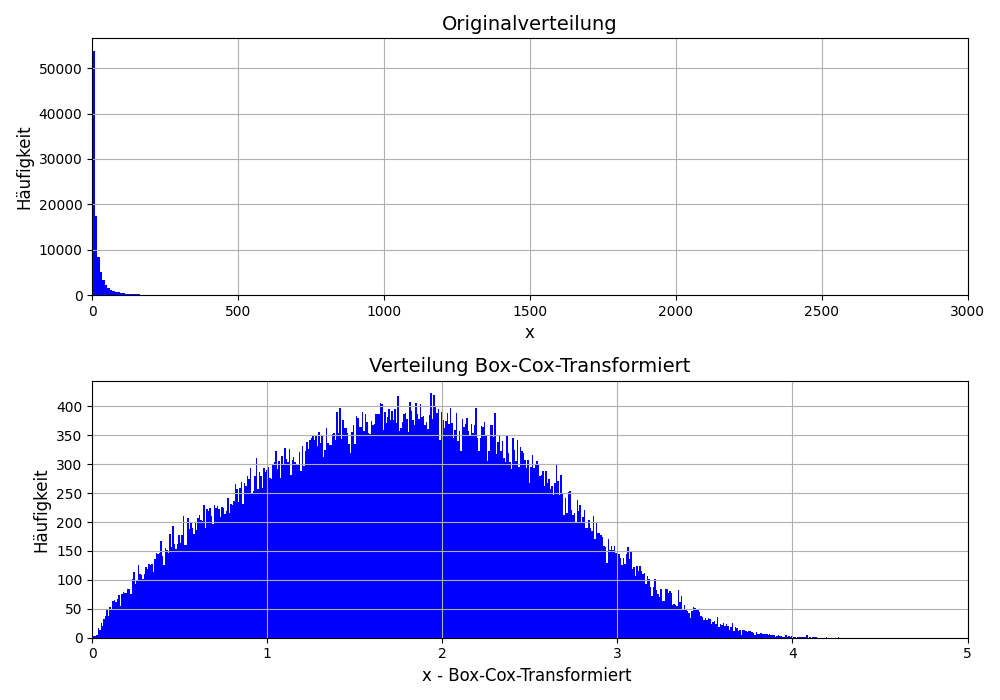
\includegraphics[width=0.9\textwidth]{img/Plots/Box-Cox-Transfomation.png}
    \caption[Beispielanwendung der Box-Cox-Transformation.]{Beispielanwendung der Box-Cox-Transformation. Werte eines \gls{Feature}[s], welche sich nicht normal verteilen. Die Anwendung verkleinert den Wertebereich erheblich und nähert die Verteilung einer Normalverteilung an.}
    \label{fig:bspBoxCox}
\end{figure}

Auch können aus bestehenden \gls{Feature}[s] neue kreiert werden. Ein Beispiel hierfür sind Interaktionsfeatures. Die einfachste Form ist die paarweise Multiplikation von \gls{Feature}[s]. Dies ist interpretierbar als eine Verknüpfung mit einem logischen UND. Dadurch entstehen neue \gls{Feature}[s] für das Modell, welche die Information von \gls{Feature}[s] enthalten, welche gerade in Kombination miteinander nützlich sind. Gerade einfachere Modelle, die eigenständig nicht so gut darin sind komplexe Zusammenhänge zu erkennen, können von dieser kombinierten Information profitieren \cite{Zheng.2018}.\par

Wird mit Sequenzen gearbeitet, dann findet in dem Prozessschritt der \gls{Feature}-Extraktion und Konstruktion ebenfalls die Konstruktion von \gls{Feature}[s] statt, welche versuchen, die Information der Sequenz zu komprimieren (\autoref{sec:sequenzen ML}) \cite{Nielsen.2020}. 

\subsection{Feature Analyse und Auswahl} \label{sec:ML FeatSelect}
Aus der Menge der \gls{Feature}[s] sind diejenigen auszuwählen, welche dem Modell übergeben werden sollen. Eine sorgfältige Auswahl der \gls{Feature}[s] ist wichtig, um ein zuverlässiges Modell zu erstellen. Hauptziel ist es, die \gls{Feature}[s] auszuwählen, mit welchen die Performance des Modells maximal wird. Ein weiteres Ziel ist die Minimierung der \gls{Feature}[anzahl], um den Rechenaufwand zu reduzieren. Eine kleinere Anzahl an \gls{Feature}[s] macht das Modell effizienter \cite{Kuhn.2013, Guyon.2003}. Wie in \autoref{sec:Herausforderungen ML} beschrieben, können \gls{Feature}[s], welche keine Information zur Erfüllung der Aufgabe besitzen, \gls{Underfitting} verursachen. Ebenfalls sind die \gls{Feature}[s] auf ungewollten \gls{Bias} zu überprüfen. Die Identifikation von ungewollten \gls{Bias} ist nicht einfach. Fachwissen und Wissen über typische Quellen von \gls{Bias} können dabei helfen \cite{Mehrabi.2019, Nielsen.2020}. In der Praxis wird zwischen drei Methoden für die Selektion von \gls{Feature}[s] unterschieden \cite{Guyon.2003}. \dubpar

\textbf{\gls{Filter Methoden}}\par
\gls{Filter Methoden} bewerten \gls{Feature}[s] Modell unabhängig und univariat. Das bedeutet, sie bewerten jedes \gls{Feature}[s] für sich. Mögliche Informationen, die durch die Kombination mehrerer \gls{Feature}[s] entstehen, werden nicht berücksichtigt. Sie vergeben für jedes \gls{Feature} eine Wertung, wodurch eine Rangfolge entsteht. Durch die univariate Bewertung können auch redundante \gls{Feature}[s] in die Auswahl aufgenommen werden, wenn sie individuell einen hohen Wert erzielen. Es gibt \gls{Filter Methoden} die auf Regressionsprobleme ausgelegt sind und Methoden, die auf \gls{Klassifikation}[sprobleme] ausgelegt sind. Da für diese Arbeit die Methoden für \gls{Klassifikation}[sprobleme] relevant sind, werden nur diese hier vorgestellt.\par

\textit{Gegenseitige Information:} Die gegenseitige Information stammt aus der Informationstheorie und ist ein Maß für die Abhängigkeit zweier Variablen. In diesem Fall zwischen den Klassen \(Y\) und einem \gls{Feature} \(X\). Die Aussage der gegenseitige Information ist, wie viel Information eine Variable über eine Andere hat. Die Formel \ref{eq:MutInfo} zeigt die Berechnung. 

\begin{equation}
I(X; Y) = \sum_{y \in Y} \sum_{x \in X} P_{X,Y}(x, y) \log \left( \frac{P_{X,Y}(x, y)}{P_X(x) P_Y(y)} \right)
\label{eq:MutInfo}
\end{equation}

Sind die Variablen unabhängig, gilt \(P(X)P(Y) = P(X,Y)\) und die gegenseitige Information ist gleich null. Besteht Abhängigkeit zwischen den Variablen ist \(I(X; Y) > 0\). Je höher die Abhängigkeit, desto größer ist \(I(X; Y)\) \cite{Cover.2006}.\par

\textit{Varianzanalyse:} Die Varianzanalyse ist eine statistische Methode. Sie überprüft, ob signifikante Unterschiede zwischen den Mittelwerten der Klassen liegen, in Bezug auf ein \gls{Feature}. Die Formeln \ref{eq:ANOVAVarZwiKla}, \ref{eq:ANOVAVarInKla} und  \ref{eq:ANOVA} zeigen die Berechnung.

\begin{equation}
Varianz\_zwischen\_den\_Klassen = \frac{\sum_{i=1}^{n} n_i(\bar{K}_i - \bar{K})^2}{(S - 1)}
\label{eq:ANOVAVarZwiKla}
\end{equation}

\begin{equation}
Varianz\_innerhalb\_der\_Klassen = \frac{\sum_{i=1}^{S} \sum_{p=1}^{n_i} (K_{ip} - \bar{K}_i)^2}{(N - S)}
\label{eq:ANOVAVarInKla}
\end{equation}

\begin{equation}
F\text{\_value} = \frac{Varianz\_zwischen\_den\_Klassen}{Varianz\_innerhalb\_der\_Klassen}
\label{eq:ANOVA}
\end{equation}

\(N\) ist die gesamte Anzahl der Proben. \(S\) ist die Anzahl an Klassen. \(n_i\) ist die Anzahl der Proben in der Klasse \(i\). \(\bar{K}_i\) ist der Mittelwert der Klasse \(i\) und \(\bar{K}\) ist der Mittelwert aller Proben. \(\bar{K}_{ip}\) ist das Element \(p\) in Klasse \(i\) \cite{Pathan.2022}. \par

Existiert keine Varianz innerhalb der Klassen, ist die Wertung null. Eine hohe Varianz in den Gruppen reduziert die Wertung und eine hohe Varianz zwischen den Gruppen erhöht die Wertung. Interpretierbar ist dies wie folgt: Umso besser sich die Klassen voneinander trennen lassen, desto besser ist die Wertung \cite{Pathan.2022, Guyon.2003}. \dubpar

\textbf{\gls{Wrapper Methoden}}\par

Anders als die \gls{Filter Methoden} treffen \gls{Wrapper Methoden} ihre Auswahl nicht univariat und auch nicht Modell unabhängig. Dadurch sind sie in der Lage, informative Kombinationen von \gls{Feature}[s] zu erkennen. Es kann auch sein, dass manche Modelle mit bestimmten \gls{Feature}[s] besser umgehen können als andere. Auch solche Einflüsse sind mit \gls{Wrapper Methoden} erkennbar \cite{Kuhn.2013, Guyon.2003}. \par

Die \gls{Wrapper Methoden} betrachten ein Modell als Blackbox. Sie entscheiden über die Eingabe in die Blackbox und beurteilen die Ausgabe von dieser. Die Ausgabe ist die Wertung einer Performancemetrik. Auf Performancemetriken wird später genauer eingegangen. Aus der Menge an \gls{Feature}[s] wird eins entnommen. Damit wird das Modell trainiert und die Performance bewertet. Wirkt sich das \gls{Feature} positiv auf die Metrik aus, dann wird es in die Auswahl aufgenommen. Wenn nicht, dann wird es zurückgelegt. Anschließend wird ein weiteres \gls{Feature} aus der Menge entnommen und in Kombination mit der bestehenden Auswahl überprüft. Wieder wird ein Modell trainiert und Performance bewertet. Dieser Prozess wird wiederholt, bis ein Abbruchkriterium erreicht ist. Dieses kann sich entweder auf die Performancemetrik beziehen, oder auf die \gls{Feature}[anzahl]. Z.B. kann das Vorgehen abgebrochen werden, wenn sich die Performance nicht mehr weiter verbessert, oder wenn eine gewünschte \gls{Feature}[anzahl] erreicht ist. Die Abbildung \ref{fig:WrapMeth} veranschaulicht das Vorgehen der \gls{Wrapper Methoden} \cite{Kuhn.2013, Guyon.2003}.

\begin{figure}[htb]
    \centering
    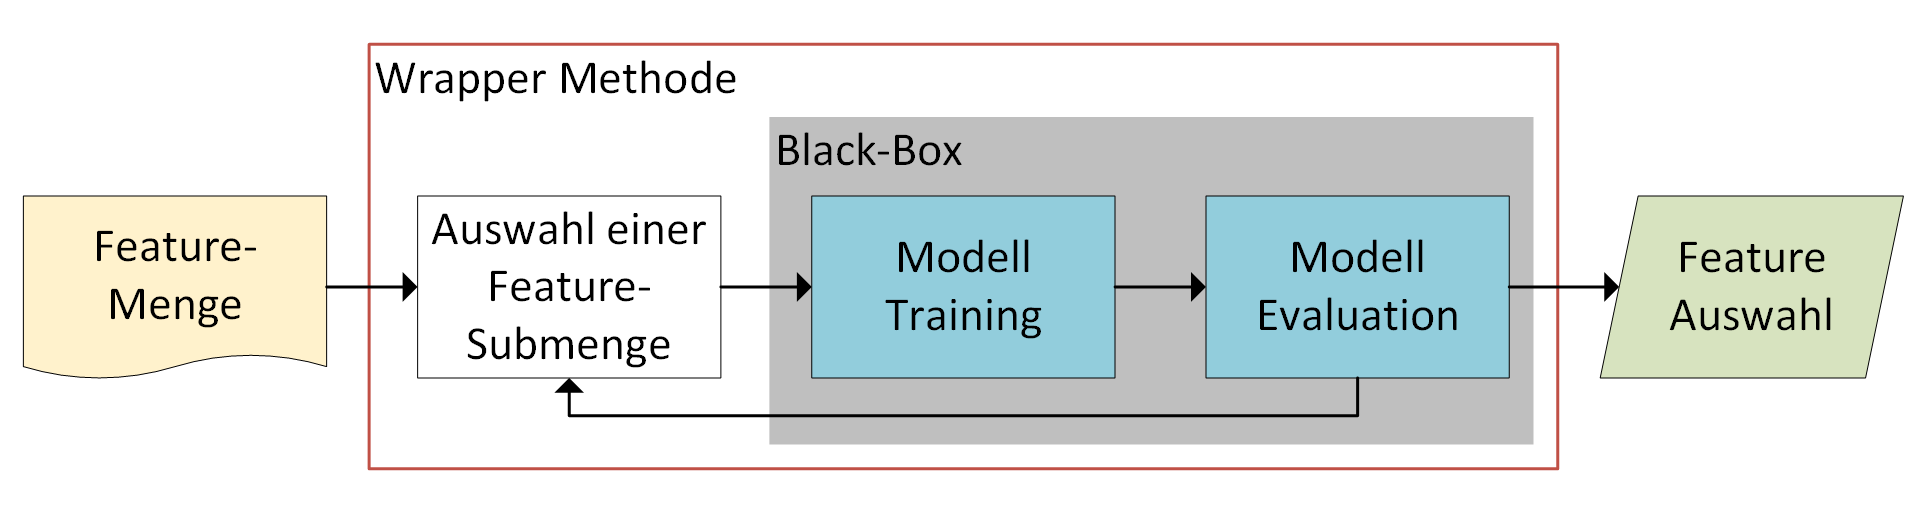
\includegraphics[width=0.9\textwidth]{img/Grafiken/Wrapper Methode bsp.png}
    \caption[Vorgehen der Wrapper Methoden.]{Vorgehen der \gls{Wrapper Methoden}. Aus der \gls{Feature}[menge] werden iterativ \gls{Feature}[s] ausgewählt und in Kombination mit der bestehenden \gls{Feature}[auswahl] evaluiert. Dazu wird das Modell in der Blackbox trainiert und die Performance bewertet.}
    \label{fig:WrapMeth}
\end{figure}

Bei den \gls{Wrapper Methoden} wird zwischen zwei Verfahren unterschieden. Der Vorwärtssuche und der Rückwärtssuche. Die Beschreibung von eben ist die der Vorwärtssuche. Bei der Rückwärtssuche befinden sich zu Beginn alle \gls{Feature}[s] in der Auswahl. Iterativ werden \gls{Feature}[s] aus der Auswahl ausgeschlossen. Dies geschieht, indem überprüft wird, wie sich der Verzicht auf ein \gls{Feature} auf die Performance auswirkt. Wirkt sich der Verzicht positiv aus, oder zumindest nicht negativ, dann wird das \gls{Feature} ausgeschlossen. Dieses Vorgehen, hat den Vorteil, dass Informationen, die in der Kombination von \gls{Feature}[s] liegen auf jeden Fall erkannt werden, da von Beginn an alle \gls{Feature}[s] zusammen bewertet werden. \dubpar

\textbf{\gls{Embedded Methoden}}\par

 \gls{Embedded Methoden} beurteilen \gls{Feature}[s], wie die \gls{Wrapper Methoden}, multivariat. Diese Auswahlmethoden sind direkt in bestimmten Modellen implementiert. Dadurch sind sie auch sehr abhängig vom Modell. Bei der linearen Regression können bspw. die Gewichte der \gls{Feature}[s] als ein Indikator für die Wichtigkeit der \gls{Feature}[s] sein. Andere Modelle implementieren diese Verfahren jedoch deutlich aussagekräftiger. Steht bereits fest, welches Modell verwendet werden soll, kann es sinnvoll sein \gls{Embedded Methoden} für die \gls{Feature}[selektion] zu verwenden, da sie eine Auswahl treffen, die sehr auf das Modell zugeschnitten ist. Steht das Modell noch nicht fest, können \gls{Feature}[s] ausgewählt werden, welche mit anderen Modellen weniger gut funktionieren \cite{Guyon.2003, Zheng.2018}.

 \subsection{Datensätze im maschinellen Lernen} \label{sec:Datensätze ML}
 Das Ergebnis der Feature-Extraktion, Konstruktion und Auswahl ist ein fertiger Datensatz, mit dem das Modell zu erstellen ist. Die Qualität und die Quantität der Daten hat dabei einen großen Einfluss auf die Performance des Modells (\autoref{sec:Herausforderungen ML}). Ziel ist es ein Modell zu entwerfen, was gut darin ist, unbekannte Proben zu schätzen. Um diese Fähigkeit zu beurteilen, werden einige Daten aus dem Datensatz zurückgehalten. Diese Daten werden nicht für das Training verwendet. Sie bleiben dem Modell unbekannt, um später die Performance auf unbekannten Daten zu beurteilen. Der Datensatz wird aufgeteilt in einen \gls{Trainingsdatensatz} und eine \gls{Testdatensatz}. Oftmals wird ein weiterer Datensatz mit Daten benötigt, die nicht für das Training verwendet werden. Dieser wird als Validierungsdatensatz bezeichnet. Der Validierungsdatensatz wird verwendet, um den Algorithmus auszuwählen und die \gls{Hyperparameter} einzustellen. Der Testdatensatz wird für den finalen Test verwendet, bevor das Modell angewendet wird \cite{Burkov.2019}. \par

 Für die Aufteilung der Daten auf die drei Datensätze gibt es keine allgemeingültige Regel. Eine gute Daumen-Regel ist 70 \% Trainingsdaten, 15 \% Validierungsdaten und 15 \% Testdaten. Es gibt Validierungsmethoden, durch die kein Validierungsdatensatz notwendig ist. Dies ist besonders praktisch, wenn die Datenmenge klein ist. Dadurch stehen mehr Daten für das Training zur Verfügung \cite{Burkov.2019}. Darauf wird später näher eingegangen. \par

 Bei Mehrklassen Klassifikation ist darauf zu achten, dass die Anzahl der Proben aus jeder Klasse ungefähr ist. Ist das nicht der Fall, handelt es sich um einen unbalancierten Datensatz. Dies kann problematisch sein, wie in \autoref{sec:Herausforderungen ML} in Bezug zu \gls{Bias} erläutert. Der Datensatz sollte balanciert werden. Eine Möglichkeit einen unbalancierten Datensatz auszubalancieren ist Undersampling. Dabei werden zufällig Proben aus den Mehrheitsklassen entfernt, bis alle Klassen ungefähr die gleiche Anzahl von Proben besitzen \cite{Burkov.2019}.


 \subsection{Auswahl des Algorithmus} \label{sec:ML ModellSelect}
 Die Auswahl des richtigen Algorithmus ist oftmals nicht einfach. Ist ausreichend Zeit, dann ist es sinnvoll mehrere Algorithmen auszuprobieren, um zu prüfen, welcher die beste Performance erzielt. Ebenfalls kann es hilfreich sein, die Auswahl anhand Kriterien einzuschränken. Die Auswahl der Kriterien geschieht anhand der Anforderungen und Randbedingung, die zum Zeitpunkt der Modellauswahl bekannt sind. Beispiele für solche Kriterien sind

 \begin{itemize}
     \item Die zur Verfügung stehende Rechenleistung.
     \item Die Geschwindigkeit der Schätzung
     \item Die zur Verfügung stehende Datenmenge
     \item Die Nachvollziehbarkeit des Schätzungsergebnisses
 \end{itemize}

 Um von den Modellen eins zu wählen, sind diese jeweils zu trainieren, einzustellen und zu validieren. Da die Einstellung der \gls{Hyperparameter} aufwendig seien kann, ist hier meistens eine grobe Einstellung ausreichend \cite{Burkov.2019, Geron.2019}.

\subsection{Überblick über Algorithmen und Modelle des maschinellen Lernens} \label{sec:ML Algorithmen}
Es existieren eine Vielzahl von Algorithmen und Modelle für \gls{ML}. Einen breiten Überblick über unterschiedliche Ansätze zu schaffen übersteigt den Rahmen dieser Arbeit. Aus diesem Grund werden hier die Funktionsprinzipien einer Auswahl von Modellen vorgestellt, die für diese Arbeit relevant sind. 

\textbf{k-Means Algorithmus} \par
k-Means ist ein Algorithmus der Clusteranalyse. Es ist eine \glsdisp{unüberwachtes Lernen}{unüberwachte Lernmethode}. Bei diesem ist der \gls{Hyperparameter} \(K\) auf die Anzahl der Klassen einzustellen, die in den Daten gefunden werden sollen. Aus dem \gls{Trainingsdatensatz} werden \(K\) zufällige Datenpunkte als Clusterzentren initialisiert. Iterativ werden nun neue Datenpunkte aus dem \gls{Trainingsdatensatz} gezogen. Die Distanz zwischen den Datenpunkten und den Clusterzentren wird ermittelt. Der Datenpunkt wird dem Cluster zugeordnet, zu dessen Zentrum die kleinste Distanz besteht. Anschließend findet eine Aktualisierung der Clusterzentren statt, indem die Mittelpunkte der Cluster berechnet werden. Die Mittelpunkte sind die neuen Zentren für die nächste Iteration \cite{Burkov.2019, Goodfellow.2016, Duda.2001}. \dubpar


\textbf{Hierarchisches Clustering} \par
Hierarchisches Clustering umfasst ebenfalls Algorithmen der Clusteranalyse. Es sind \glsdisp{unüberwachtes Lernen}{unüberwachte Lernmethoden}. Anders als bei k-Means ist keine \gls{Hyperparameter}[einstellung] der Clusteranzahl notwendig. Ansatz von hierarchischen Clustering Methoden ist, dass sich viele Cluster in Subcluster unterteilen lassen, welche sich ebenfalls in Subcluster unterteilen lassen. Als Beispiel wird ein Cluster \textit{Tiere} genommen. Dieses kann unterteilt werden in \textit{Säugetiere} und \textit{Reptilien}. Das Cluster \textit{Säugetiere} ist weiter unterteilbar in \textit{Fleischfresser} und \textit{Pflanzenfresser}. Hierarchisches Clustering versucht solche hierarchischen Strukturen zu modellieren. Dazu gibt es zwei Verfahren: agglomeratives  Clustering und divisives Clustering. Beim agglomerativen Clustering startet jeder Datenpunkt als eigenes Cluster. Bei jeder Iteration werden die beiden Cluster, die am nächsten zueinander liegen, zu einem Cluster zusammengefasst. Dadurch entsteht eine Baumstruktur. Der Anwender kann entscheiden, welche hierarchische Ebene die Aufgabe am besten modelliert und kann die Struktur an dieser Stelle auftrennen. Das diversive Clustering funktioniert genau andersherum. Alle Daten starten in einem großen Cluster. Die Subcluster, welche sich am unähnlichsten sind, werden in der nächsten Stufe aufgeteilt \cite{Duda.2001}. Die Abbildung \ref{fig:HiraClust} zeigt die beim hierarchischen Clustering entstehende Baumstruktur beispielhaft. 

\begin{figure}[htb]
    \centering
    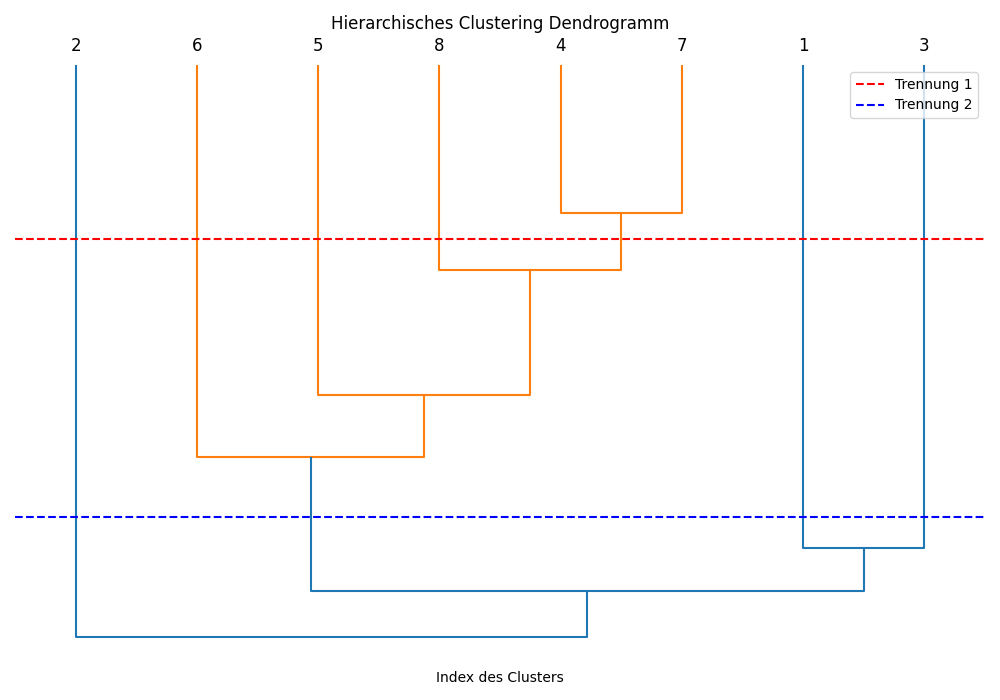
\includegraphics[width=0.9\textwidth]{img/Plots/Dendogramm Hierachisches Clustering.png}
    \caption[Dendrogramm zu einem Beispiel des Hierarchisches Clusterings.]{Dendrogramm zu einem Beispiel des Hierarchisches Clusterings. Die horizontalen Linien zeigen, dass über die Cluster-Anzahl entschieden werden kann, durch die Wahl der Trennebene.}
    \label{fig:HiraClust}
\end{figure}

\dubpar
\textbf{Logistische Regression} \par
\begin{wrapfigure}{l}{0.4\textwidth}
    \begin{center}
        \vspace*{-7mm}
        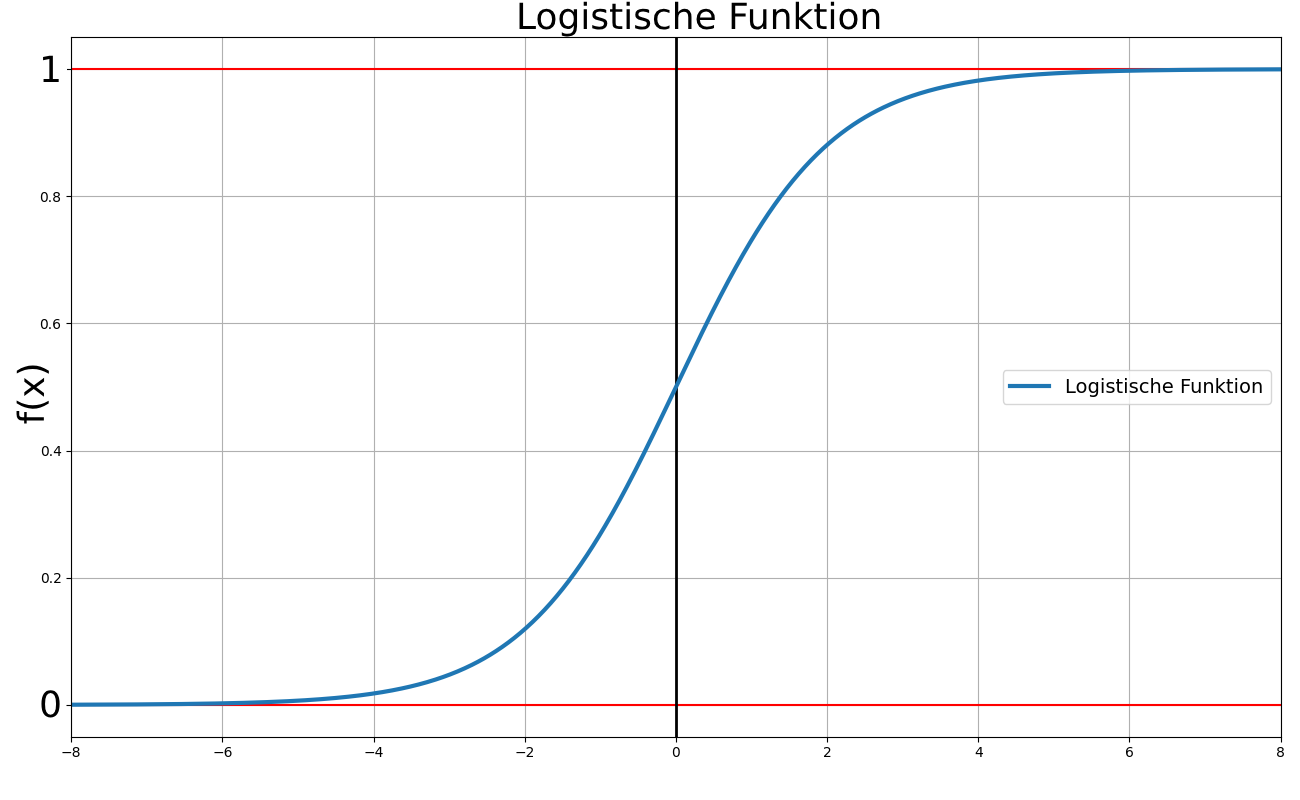
\includegraphics[width=0.4\textwidth, height=4cm]{img/Plots/Logistische Funktion.png}
        \vspace*{-10.5mm}
        \caption[Verlauf der logistischen Funktion.]{Verlauf der logistischen Funktion.}
        \label{fig:LogiFunc}
    \end{center}
\end{wrapfigure}
Die logistische Regression ist ein \gls{Klassifikation}[salgorithmus], auch wenn der Name anderes vermuten lässt. Es handelt sich um einen \glsdisp{überwachtes Lernen}{überwachten Algorithmus} für binäre \gls{Klassifikation} (\autoref{sec:ML klass und Reg}). Die logistische Regression verwendet die logistische Funktion aus der \autoref{eq:LogiFunc} (einen Spezialfall der Sigmoidfunktion), um Daten binär \((0,1)\) zuzuordnen. Die Abbildung \ref{fig:LogiFunc} zeigt den Verlauf der logistischen Funktion \cite{Burkov.2019}. 

\begin{equation}
f(x) = \frac{1}{1 + e^{-x}}
\label{eq:LogiFunc}
\end{equation}

Die logistische Regression trägt das Wort \textit{Regression} im Namen, da es verwandt ist mit der linearen Regression. Die Modellformulierung ist so interpretierbar, dass ein lineares Regressionsmodell, auf einen Wertebereich von \((0,1)\) abgebildet wird. Die Modellformulierung ist in \autoref{eq:LogiReg} zu sehen.

\begin{equation}
\hat{y}_{\nomvec{w},b}(\nomvec{x}) = \frac{1}{1 + e^{-(\nomvecT{w}\nomvec{x})+\nomvec{b})}}
\label{eq:LogiReg}
\end{equation}

Wird eine Probe geschätzt und erhält einen Wert \(\hat{y}_{\nomvec{w},\nomvec{b}}(\nomvec{x}) > 0,5\) dann wird die Probe der Klasse \(1\) zugeordnet. Ist \(\hat{y}_{\nomvec{w},\nomvec{b}}(\nomvec{x}) < 0,5\), dann gehört die Probe in die Klasse \(0\) \cite{Burkov.2019, Goodfellow.2016}.

\dubpar
\textbf{Support Vector Machine (\acrshort{SVM})} \par
Eine \acrshort{SVM} ist ein Modell des \glsdisp{überwachtes Lernen}{überwachten Lernens} für binäre \gls{Klassifikation}. Es versucht die Datenpunkte im \gls{Feature}[raum] mittels einer Hyperebene zu separieren. Die Hyperebene wird als Entscheidungsgrenze bezeichnet. Die Punkte aus jeder Klasse, welche am nächsten zu der Entscheidungsgrenze liegen, werden als Support Vektoren bezeichnet. Mittels diesen wird die Entscheidungsgrenze so ausgerichtet, dass sie möglichst gleich weit entfernt von allen Support Vektoren verläuft. Im Trainingsprozess versucht die \acrshort{SVM} somit die maximale Abgrenzung zwischen den Klassen zu finden. Die Abbildung \ref{fig:bspLinSVM} veranschaulicht das Konzept der Entscheidungsgrenze und den Support Vektoren. 

\begin{figure}[htb]
    \centering
    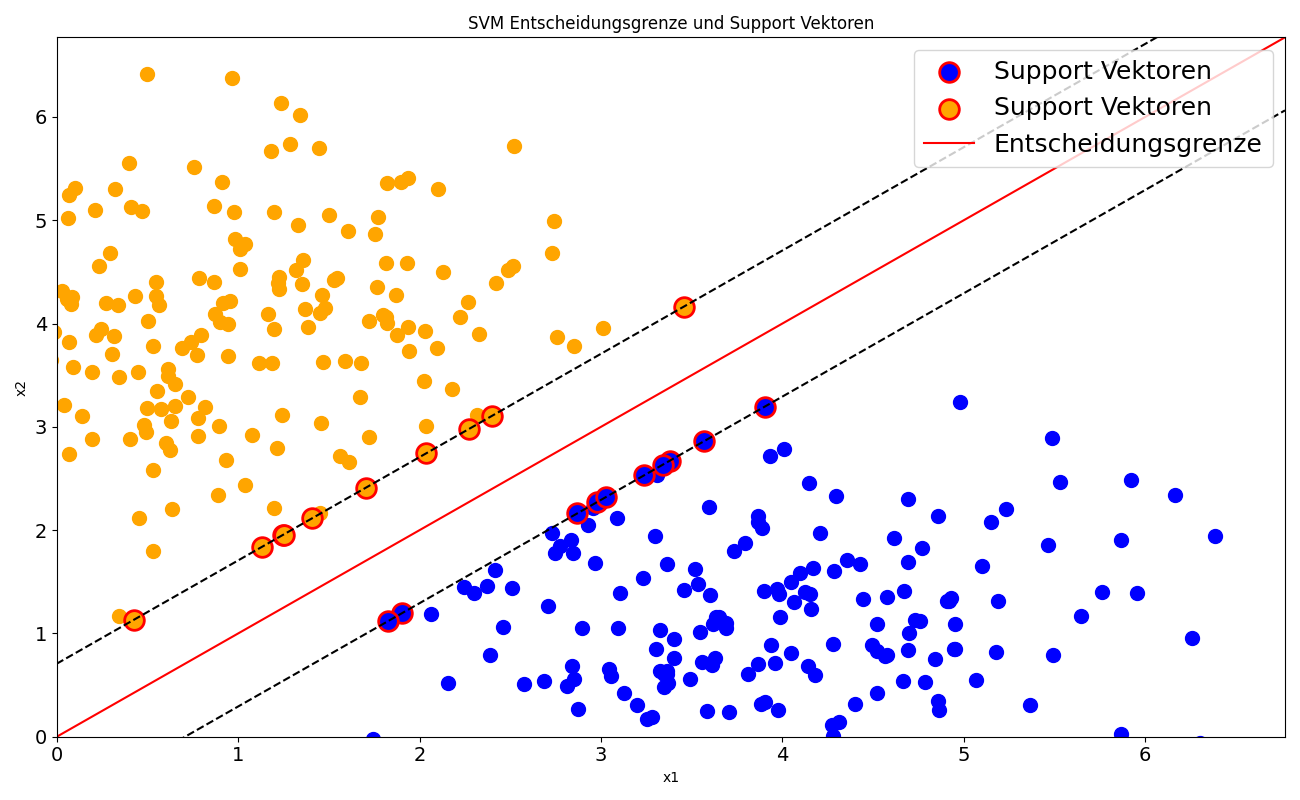
\includegraphics[width=0.9\textwidth]{img/Plots/SVM Beispiel.png}
    \caption[Beispiel der Funktionsweise einer SVM.]{Beispiel der Funktionsweise einer SVM. Anhand der Support Vektoren wird die Entscheidungsgrenze so ausgerichtet, dass sie gleich weit von beiden Klassen entfernt verläuft.}
    \label{fig:bspLinSVM}
\end{figure}

Definiert wird die Entscheidungsgrenze nach der Koordinatenform, wie die Gleichung \ref{eq:SVMdefHypEb} zeigt.

\begin{equation}
\nomvecT{w}\nomvec{x}+\nomvec{b}=0
\label{eq:SVMdefHypEb}
\end{equation}

Die Modellfunktion evaluiert die Klassenzugehörigkeit, indem sie überprüft, ob sich ein Datenpunkt oberhalb, oder unterhalb der Entscheidungsebene befindet. Dies erfolgt, indem der Datenpunkt in die Ebenengleichung eingesetzt wird. Anschließend gibt das Vorzeichen die Klassenzugehörigkeit an. Das ist in der Gleichung \ref{eq:SVMmodell} zu sehen. 

\begin{equation}
\hat{y}_{\nomvec{w},\nomvec{b}}(\nomvec{x}) = sgn(\nomvecT{w}\nomvec{x}+\nomvec{b}))
\label{eq:SVMmodell}
\end{equation}

Das Modell der Gleichung \ref{eq:SVMmodell} wird im Allgemeinen als lineare \acrshort{SVM} bezeichnet. Es gibt auch Verfahren, mit denen nicht-lineare Entscheidungsgrenzen verwendet werden können \cite{Burkov.2019, Goodfellow.2016, ShalevShwartz.2014}. \dubpar

\textbf{Random Forest}\par
Der Random Forest Algorithmus gehört zu den \glsdisp{überwachtes Lernen}{überwachten Lernverfahren} und ist eine Ensemble-Methode. Ensemble-Methoden nutzen ein Ensemble aus mehreren einfachen Modellen für ihre Entscheidungsfindung. Der Random Forest Algorithmus besteht aus mehreren Entscheidungsbäumen. Ein Entscheidungsbaum ist ein grafischer Ansatz für \gls{ML}. In einem Beispiel ist der Wert eines Autos zu schätzen. Ein Entscheidungsbaum betrachtet in den Knoten die \gls{Feature}[s] und entscheidet sich auf Basis von Schwellwerten, welcher Kante er folgt. Bezogen auf das Beispiel wird in einem Knoten überprüft, ob das Auto älter oder jünger als 10 Jahre ist. Beim Erreichen der Blätter des Baumes wird eine Entscheidung getroffen. Während des Trainings versucht ein Baum funktionierende Schwellwerte in den Knoten zu finden. Entscheidungsbäume eignen sich für die \gls{Klassifikation}, sowie die Regression. Auch Mehrklassenprobleme sind ohne weiteres mit Entscheidungsbäumen lösbar \cite{Burkov.2019, Bishop.2006, Goodfellow.2016}. \par

Der Random Forest Algorithmus zieht aus dem \gls{Trainingsdatensatz} eine zufällige Menge an Proben mit zurücklegen. Damit wird ein einzelner Baum trainiert. In den verschiedenen Knoten wird immer nur eine zufällige Teilmenge der \gls{Feature}[s] berücksichtigt. Durch diese Zufallsmechanismen wird gewährleistet, dass die resultierenden Bäume unterschiedlich sind. Das Modell schätzt eine unbekannte Probe, indem sie von allen Entscheidungsbäumen evaluiert wird. Das finale Ergebnis entsteht durch eine Mehrheitsentscheidung. Typische \gls{Hyperparameter} von  Random Forest Algorithmen sind die Anzahl der Bäume und die Baumtiefe \cite{Burkov.2019, Breiman.2001}. \dubpar

\textbf{Gradient Boosting} \par
Gradient Boosting gehört zu den \glsdisp{überwachtes Lernen}{überwachten Lernverfahren} und ist ebenfalls eine Ensemble-Methode, die auf Entscheidungsbäumen beruht. Während Random Forest seine Entscheidungsbäume unabhängig und parallel aufbaut, erstellt Gradient Boosting diese sequenziell. \par 

Zu Beginn wird ein konstanter Entscheidungsbaum initialisiert. Dieser ist die Ausgangssituation für die Modellierung mit Entscheidungsbäumen. Es existiert ein einziger Knoten, welcher auf jede Eingabe identisch bewertet. Mit diesem konstanten Entscheidungsbaum werden alle Proben im \gls{Trainingsdatensatz} bewertet. Anschließend wird die Abweichung gemessen. Diese Abweichung wird für den nächsten Entscheidungsbaum als \gls{Label} für die Daten verwendet. Der folgende Baum lernt somit die Fehler seines vorausgegangenen Baumes zu schätzen. Sequentiell lernen die folgenden Bäume den verbleibenden Fehler zu schätzen. \par

Ist eine unbekannte Probe zu schätzen, weiß das Modell nach dem Training, wie es die Fehler in den Bäumen korrigieren muss. Ein wichtiger \gls{Hyperparameter} im Gradient Boosting ist die Lernrate. Diese bestimmt die Stärker der Korrektur für jede Stufe in der Sequenz. Ist bspw. laut Entscheidungsbaum die Schätzung um den Wert \(a\) zu korrigieren, sorgt die Lernrate \(\alpha\) dafür, dass die Schätzung nur um \(\alpha \cdot a\) korrigiert wird. Dies kann Overfitting vermeiden \cite{Burkov.2019}. \par

Eine Variante des Gradient Boosting wird als histogrammbasiertes Gradient Boosting bezeichnet. Bei dieser werden die Features zuvor gruppiert, ähnlich der Gruppierung bei der Feature-Konstruktion (\autoref{sec:ML FeatExtr}). Dadurch wird die Anzahl unterschiedlicher Werte reduziert. Das Gradient Boosting ist somit effizienter durchzuführen \cite{Ke.2017}. 
\dubpar


\textbf{Long Short-Term Memory (\acrshort{LSTM})} \par
\acrshort{LSTM}[s] sind Modelle des \gls{Deep Learning}. Sie sind eine spezielle Form von rekurrenten neuronalen Netzwerken (\acrshort{RNN}[s]). \acrshort{RNN}[s] sind darauf ausgelegt Sequenzen verstehen zu können. Dies wird durch Rückführungen erreicht. Die Einheiten in den Schichten eines \acrshort{RNN}[s] besitzen einen Zustandsspeicher. Als Eingabe erhält eine Einheit die Ausgabe der vorherigen Schicht, und die Rückführung des eigenen Zustandsspeichers. Das Ergebnis aktualisiert den Zustandsspeicher. Somit wirken frühere Zeitschritte in den Daten auf spätere, wodurch Mustererkennung in Sequenzen möglich wird.\par

Es existieren jedoch einige Komplikationen klassische \acrshort{RNN}[s] anzuwenden. Aus diesem Grund haben sich sogenannte \textit{Gated \acrshort{RNN}[s]} für die Realisierung durchgesetzt. Ein solches \acrshort{RNN} ist das \acrshort{LSTM}. Die Kernidee von \acrshort{LSTM}[s] ist eine Regulierung des Zustandsspeichers der Einheiten. Der Zustandsspeicher wird durch drei Arten von Toren reguliert. Einem Eingangstor, einem Vergesstor und einem Ausgangstor. Diese Struktur ermöglicht es, Informationen über lange Zeiträume zu speichern, irrelevant gewordene Informationen zu vergessen und den Informationsfluss innerhalb der Zelle zu regulieren.

\begin{itemize}
    \item Das Eingangstor steuert, welche neuen Informationen zu einem Zeitpunkt in den Zustandsspeicher aufgenommen werden.
    \item  Das Vergesstor entscheidet, welche Teile des aktuellen Zustands erhalten bleiben oder verworfen werden.
    \item Das Ausgangstor bestimmt, welche Informationen aus dem Zustandsspeicher an den Ausgang weitergegeben werden.
\end{itemize}

Diese Mechanismen erlauben es \acrshort{LSTM}[s]s, sowohl kurzfristige als auch langfristige Datenabhängigkeiten zu lernen und effektiv zwischen relevanten und irrelevanten Informationen zu unterscheiden \cite{Burkov.2019, Goodfellow.2016}. \par

\textbf{Gated Recurrent Unit (\acrshort{GRU})}
Die \acrshort{GRU} lässt sich als vereinfachte Form eines \acrshort{LSTM}[s] betrachten. Sie verwendet ebenfalls Tore für die Handhabung langfristiger und kurzfristiger Abhängigkeiten in sequenziellen Daten. \acrshort{GRU}[s] vereinfachen die Struktur von \acrshort{LSTM}[s], indem sie nur zwei Tore verwenden. Ein Update-Tor und ein Reset-Tor. \par

\begin{itemize}
    \item Das Update-Tor entscheidet, inwieweit der aktuelle Zustandsspeicher durch den neuen Zustand ersetzt werden soll. Es ermöglicht die Dauer zu bestimmen, wie lange Information bewahrt wird.
    \item Das Reset-Tor ermöglicht es zu entscheiden, wie viel vom aktuelle Zustandsspeicher verwendet werden soll, um den neuen Zustand zu berechnen.
\end{itemize}

\acrshort{GRU}[s] sind einfacher zu trainieren als \acrshort{LSTM}[s] und sie können ähnlich gut in ihrer Performance sein \cite{Lazzeri.2021, Goodfellow.2016}. 



\subsection{Training und Validierung des Modells} \label{sec:ML Metriken, Valid}
Das Modell wird mit der \gls{Trainingsdatensatz} trainiert. Dieser Prozess ist modellabhängig. Die meisten \gls{Bibliothek}[en], die Algorithmen für \gls{ML} implementieren, haben automatische Routinen um die Modelle zu trainieren. Nach dem Training wird die Performance mit dem Validierungsdatensatz beurteilt \cite{Burkov.2019, Geron.2019, Zheng.2015}. Für die Performancebewertung existieren verschiedene Methoden. Hier werden zwei vorgestellt. \dubpar

\textbf{\gls{Accuracy}}\par

Die \gls{Accuracy} berechnet sich für ein \gls{Klassifikation} [sproblem] aus dem Verhältnis der Anzahl der richtig \glsdisp{Klassifikation}{klassifizierten} Proben \(TP\) und der Gesamtanzahl der Proben \(N\). Dies zeigt die Formel \ref{eq:MLaccuracy} \cite{Zheng.2015}.

\begin{equation}
Accuracy = \frac{|TP|}{|N|}
\label{eq:MLaccuracy}
\end{equation}

\textbf{\gls{Konfusionsmatrix}}\par
Eine \gls{Konfusionsmatrix} bietet Einblick in die Fehler, die das Modell macht. Sie zeigt, welche Verwechslungen stattfinden. In einem Beispiel wird die Performance eines Spam-Filters beurteilt. Dieser wurde mit 200 E-Mails validiert. Die Tabelle \ref{tab:bspConfMat} zeigt die \gls{Konfusionsmatrix} des Spam-Filters \cite{Zheng.2015}.

\begin{table}[h]
    \centering
    \begin{tabular}{|l|c|c|}
        \hline
                                    & Schätzung: \textit{Spam} & Schätzung: \textit{kein Spam}\\
        \hline
        Label: \textit{Spam}        & 80 & 15 \\
        \hline
        Label: \textit{kein Spam}   &  5 & 100\\
        \hline
    \end{tabular}
    \caption{\gls{Konfusionsmatrix} eines Spam-Filters. Der Filter wurde mit 200 Proben evaluiert. 80 E-Mails sind korrekt als \textit{Spam} erkannt worden und 100 korrekt als \textit{kein Spam}. 5 E-Mails wurden fälschlicherweise als \textit{Spam} geschätzt und 15 fälschlicherweise als \textit{kein Spam}.}
    \label{tab:bspConfMat}
\end{table}

Wie bereits in \autoref{sec:Datensätze ML} erwähnt, ist es möglich den Validierungsdatensatz einzusparen. Das ist mit dem Verfahren \gls{Cross-Validation} möglich. Dabei wird der \gls{Trainingsdatensatz} in \(K\) gleich große Teile aufgeteilt. Anschließend werden \(K\) Modelle trainiert, dabei wird immer ein anderes Teil des \gls{Trainingsdatensatz}[es] zurückgehalten und für die Validierung verwendet. Somit existieren \(K\) Beurteilungen der Performance. Die Gesamtperformance ist der Mittelwert. Das Modell wird anschließend mit dem vollständigen \gls{Trainingsdatensatz} trainiert. Die Abbildung \ref{fig:CrossVal} veranschaulicht die \gls{Cross-Validation}.

\begin{figure}[htb]
    \raggedright
    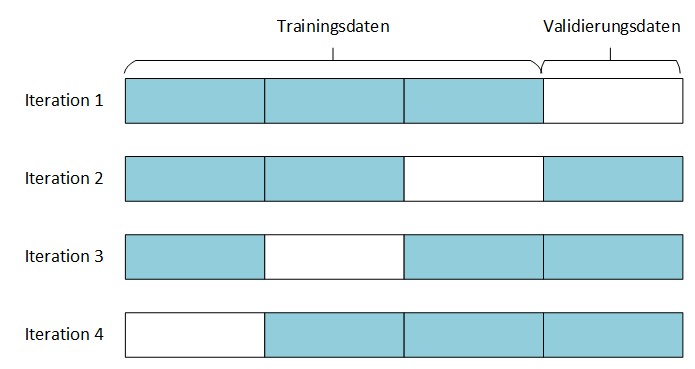
\includegraphics[width=0.9\textwidth]{img/Grafiken/Cross Validation.png}
    \caption[Verfahren der Cross-Validation.]{Verfahren der \gls{Cross-Validation}.  Der \gls{Trainingsdatensatz} wird in 4 Teile zerteilt, wovon jedes einmal als Validierungsdatensatz verwendet wird.}
    \label{fig:CrossVal}
\end{figure}

\subsection{Einstellung der Hyperparameter} \label{sec:ML HyperPara}
\gls{Hyperparameter} ermöglichen es Einfluss auf den Trainingsprozess eines Modells zu nehmen. Sie sind vor dem Training vom Anwender einzustellen. Ein Beispiel ist ein \gls{Regularisierung}[stherm]. Die Einstellung der \gls{Hyperparameter} ist sehr aufgabenspezifisch. Es gibt keine allgemeine Regel für optimale \gls{Hyperparameter}. Es ist ein Optimierungsproblem, welches sich mittels Algorithmen lösen lässt. Ziel der Optimierung ist die Maximierung des Validierungsergebnisses \cite{Zheng.2015}.\dubpar


\textbf{Grid Search}\par

Für alle \gls{Hyperparameter} wird ein Raster angegeben, z.B. für den \gls{Regularisierung}[stherm] \(C = \{0,1,1,10,100,1000\}\). Für jede Kombination von Werten der \gls{Hyperparameter} wird ein Modell trainiert und validiert. Am Ende werden die \gls{Hyperparameter} eingestellt, mit denen die beste Performance erzielt wurde. Diese Methode kann sehr rechenaufwändig sein, da jegliche Kombinationen zu prüfen sind. Gerade bei sehr feinen Rastern kann das Vorgehen viel Zeit in Anspruch nehmen \cite{Zheng.2015}.\dubpar

\textbf{Random Search}\par

Beim Random Search Verfahren bekommen die \gls{Hyperparameter} eine Wahrscheinlichkeitsverteilung zugewiesen, aus welcher diese ihre Einstellungswerte ziehen. Es wird eine festgelegte Anzahl an Kombinationen getestet. Bei jeder Iteration werden neue Zufallswerte gezogen. Dadurch ist der Rechenaufwand deutlich leichter zu überschauen als bei der Grid Search. Mit Random Search sind ähnlich gute Ergebnisse zu erzielen, wie mit Grid Search \cite{Zheng.2015, Burkov.2019}.


\subsection{Testen und Anwenden des Modells}
Die finalen Prozessschritte im \gls{Machine Learning Workflow} sind das Testen mit dem \gls{Testdatensatz} und die Integration des Modells in die Anwendung. Für das Testen werden die gleichen Metriken verwendet wie bei der Validierung (\autoref{sec:ML Metriken, Valid}). Ist der finale Test zufriedenstellend, kann das Modell in die Anwendung integriert werden. Ist dies nicht der Fall, ist eine Rückkehr zu früheren Prozessschritten notwendig \cite{Zheng.2015, Burkov.2019}.